\documentclass[reprint,aip]{revtex4-1}
\usepackage[utf8]{inputenc}
\usepackage[T1]{fontenc}
\usepackage{libertine}
\usepackage{hyperref}
\usepackage{blindtext}
\usepackage{easylist}
\usepackage{amsmath}
\usepackage{amsfonts}
\usepackage{graphicx}
\usepackage[finnish,english]{babel}
\usepackage[fixlanguage]{babelbib}
\selectbiblanguage{english}

\begin{document}

\title{Documentation for Data Structures Project}
\date{\today}
\author{Niko Ilomäki}
\email[]{niko.ilomaki@helsinki.fi}
\affiliation{University of Helsinki}

\maketitle

\section{Description}

Subject of the project is Mersenne Twister (MT), the most commonly used modern pseudorandom number generator (prng; \url{http://en.wikipedia.org/wiki/Mersenne_twister}). Implementation uses Python 3. Implementation includes a number of variants of MT, including at least MT19937 and MT19937-64 (see link above). One or more older prng's are used as reference points.

Implementation includes functions for generating numbers from the most common probability distributions, i.e. uniform, normal, exponential, binomial and beta distributions etc. Some visualization tools for the distributions will be provided. A number of randomness tests are also part of the project. These may include some of the so-called diehard tests (\url{http://en.wikipedia.org/wiki/Diehard_tests}).

MT only uses basic arrays, so no special data structures will be implemented as part of the project. Since MT is a prng, its only parameters are the size of the random number array and the used seed value. In this project, different distributions are provided as well in addition to uniform. Time usage of MT is $\mathcal{O}(n)$ where $n$ is the size of the requested random number array.

\section{Week 1}

I'll properly start the project next week; therefore this week didn't provide much new. Nothing seems unreasonably unclear at the moment and in case problems arrive I will turn to IRC first. The program itself hasn't progressed at all yet; I've researched the algorithms, but haven't coded anything. However, by next Sunday I'm aiming for a preliminary complete program. Next thing I'm going to do is implementing MT19937 and some of the distribution transform functions with Python 3.

\section{Week 2}

Lately I've been studying both Mersenne twister implementation and different probability distributions. Generators MT19937 and MT19937-64 have now been implemented in the program. A few more will follow for comparison purposes, perhaps a lagged Fibonacci generator (simpler and less random) and the Blum Blum Shub generator (very slow, but a lot better for cryptographical purposes). Most of the planned probability distributions have also been implemented. Their implementation uses quantile functions (inverse functions of the respective cumulative distribution functions) on input numbers between 0 and 1 from the generators. This is a well-known technique in Monte Carlo simulation. Output visualization and testing are priorities for next week.

\section{Week 3}

This week's additions include visualization and demos that utilize it. Quite a lot was left for the last week though some additional methods are already work in progress. Randomness, performance and bug testing will follow, as well as additional generators.

\section{Week 4}

\subsection{Quality}

Quality of pseudorandom numbers in terms of average (expectation) and variance was tested. A sample of 100 000 pseudorandoms was produced with each generators with distribution normal(0,1) and seed value 0x123456. Thus, the average should be 0 and variance 1.

\begin{table}[h]
\begin{tabular}{c|c|c}
Generator & Average & Variance \\
MT19937 & 0.00164 & 1.00441 \\
MT19937\_64 & 0.00555 & 1.00130 \\
ALFG & 0.00232 & 1.00536 \\
LCG & -0.00372 & 0.99433 \\
BBS & 0.00297 & 1.00297 \\
\end{tabular}
\caption{Average and variance}
\end{table}

All generators performed reasonably well in this sense.

Tests such as the Diehard tests were intended, but turned out to be too difficult to implement. The tests generally indicate that a certain distribution should be achieved with certain process, but testing whether an empirical distribution is 'close enough' to a theoretical distribution would require a whole new set of tools and for that there wasn't enough time in the end. Pictures are below.

\subsection{Performance}

\begin{table}[h!]
\begin{tabular}{c|c|c|c|c|c}
Generator & 1k & 2k & 4k & 8k & 16k \\
MT19937 & 1.066 & 1.893 & 3.083 & 5.857 & 11.624 \\
MT19937\_64 & 0.720 & 1.086 & 1.761 & 3.170 & 5.706 \\
ALFG & 0.461 & 0.525 & 0.652 & 0.882 & 1.362 \\
LCG & 1.062 & 1.775 & 3.229 & 5.438 & 10.858 \\
BBS & 0.526 & 0.488 & 0.557 & 0.712 & 1.010 \\
\end{tabular}
\caption{Execution time in seconds}
\end{table}

All generators performed in essentially linear time as expected. The difference in performance between the MT variants is quite puzzling because there is no apparent reason for it. Even weirder was that BBS produced 2k numbers faster than 1k, but subsequent tries proved it to be just stochastic variation. Blum Blum Shub is actually a notoriously slow generator, but that didn't show here because the primes used were only roughly $10^8$ in size. Industrial implementations would use much larger primes.

\subsection{Unit testing}

There aren't any unit tests which is partially due to the nature of the project: there wasn't anything that clearly would've needed one.

\subsection{Usage}

The project is intended to be used as a library rather than a program in itself. Any generator can be paired with any distribution. Usage is demonstrated in the demo file.

\subsection{Pictures}

Normal distribution with different generators and birthday spacings with different generators (should be exponentially distributed).

\begin{figure}[h]
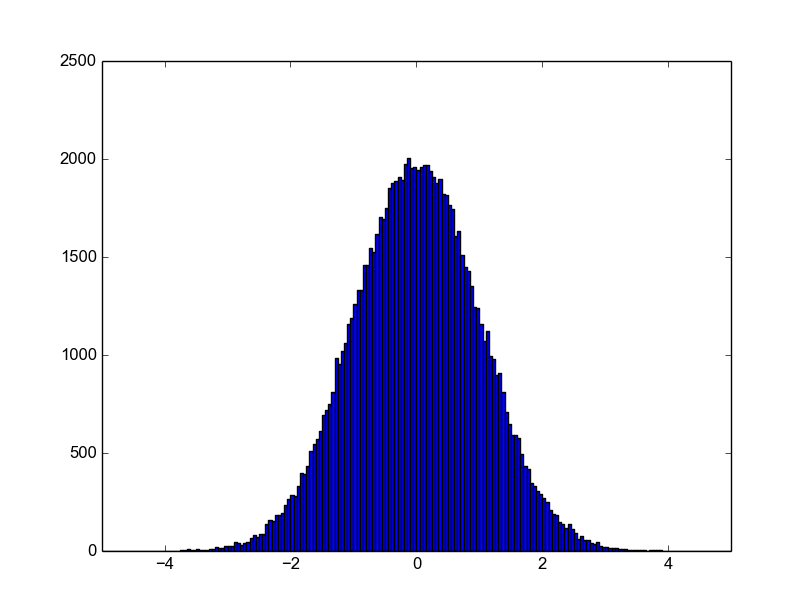
\includegraphics{normal-mt19937.png}
\caption{MT19937, normal distribution}
\end{figure}

\begin{figure}[h]
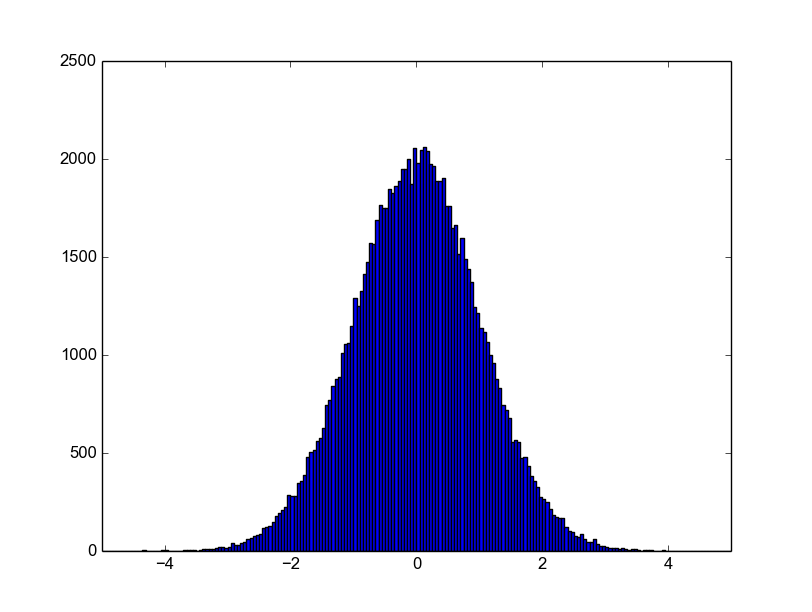
\includegraphics{normal-mt19937_64.png}
\caption{MT19937\_64, normal distribution}
\end{figure}

\begin{figure}[h]
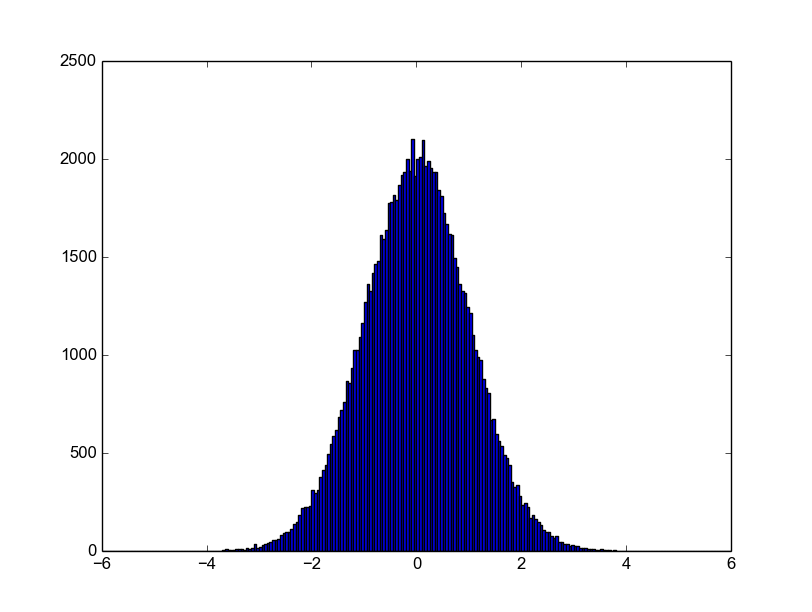
\includegraphics{normal-alfg.png}
\caption{ALFG, normal distribution}
\end{figure}

\begin{figure}[h]
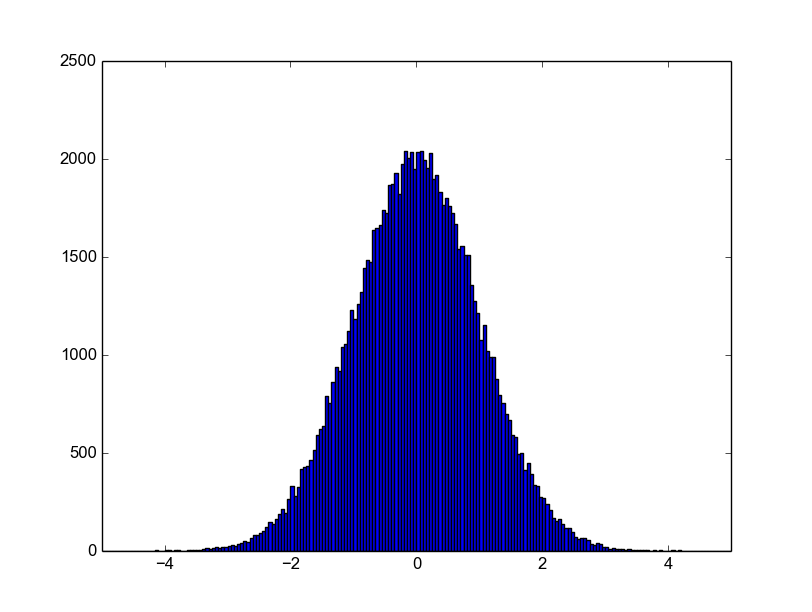
\includegraphics{normal-lcg.png}
\caption{LCG, normal distribution}
\end{figure}

\begin{figure}[h]
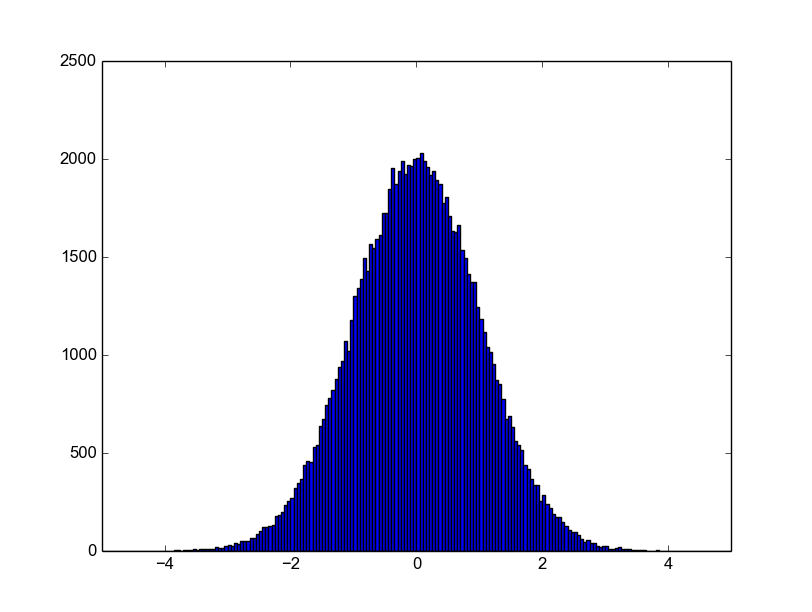
\includegraphics{normal-bbs.png}
\caption{BBS, normal distribution}
\end{figure}

\begin{figure}[h]
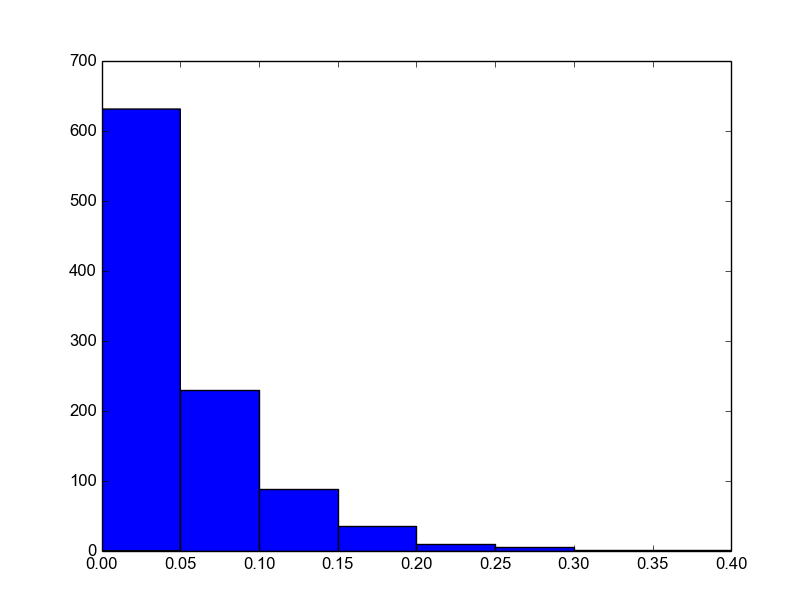
\includegraphics{bday-mt19937.png}
\caption{MT19937, 'birthday' spacings}
\end{figure}

\begin{figure}[h]
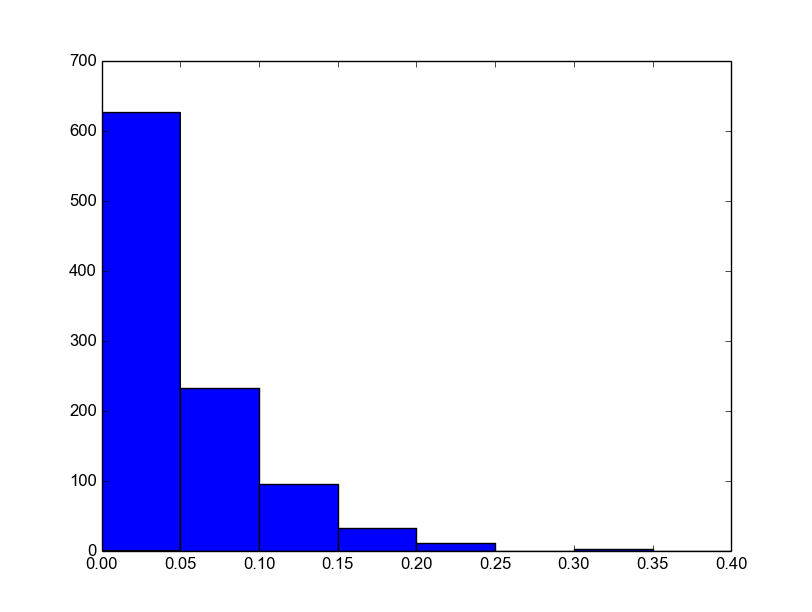
\includegraphics{bday-mt19937_64.png}
\caption{MT19937\_64, 'birthday' spacings}
\end{figure}

\begin{figure}[h]
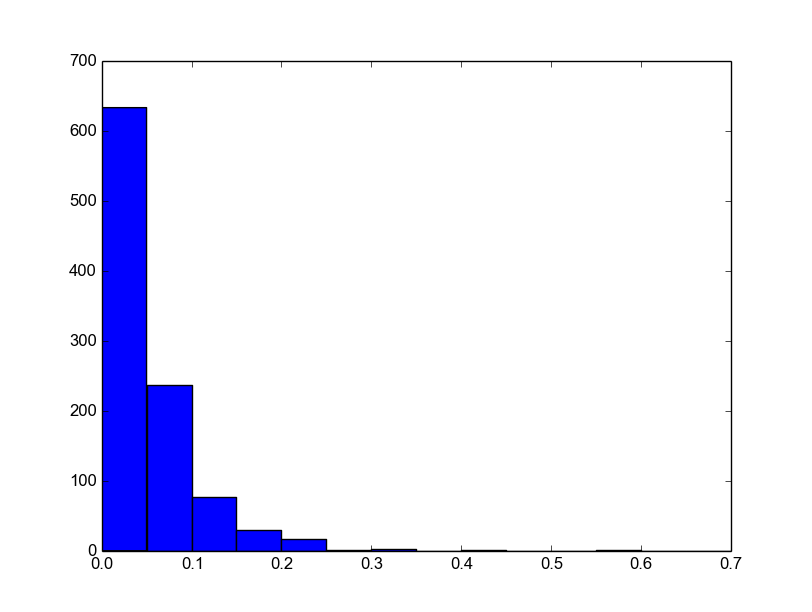
\includegraphics{bday-alfg.png}
\caption{ALFG, 'birthday' spacings}
\end{figure}

\begin{figure}[h]
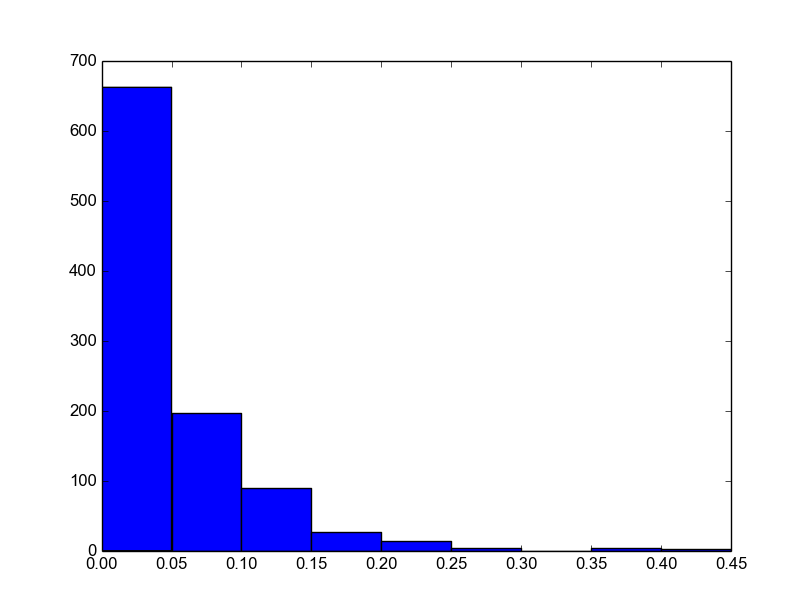
\includegraphics{bday-lcg.png}
\caption{LCG, 'birthday' spacings}
\end{figure}

\begin{figure}[h]
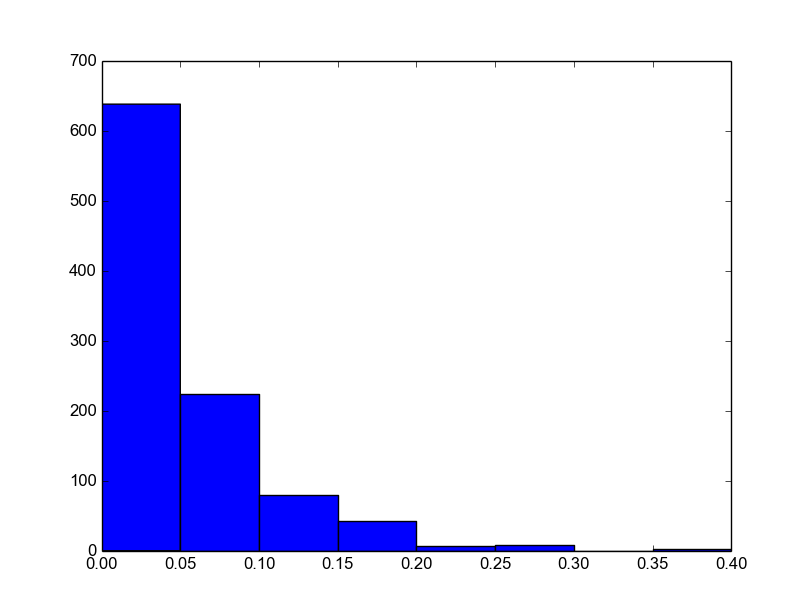
\includegraphics{bday-bbs.png}
\caption{BBS, 'birthday' spacings}
\end{figure}


\end{document}
